\subsection{Panel trenera personalnego}\label{subsec:panel-trenera-personalnego}

{\includegraphics{diagrams/use_cases/trener_personalny}}
{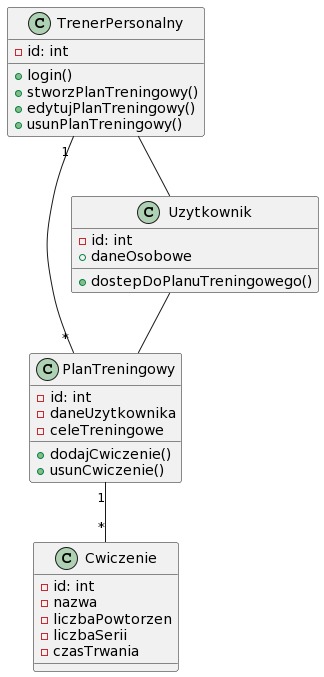
\includegraphics{diagrams/class/trener_personalny_klasy}}

\begin{enumerate}
\tightlist
\item
  {Stwórz plan treningowy}
\end{enumerate}

{\includegraphics{diagrams/sequence/tworzenie_planu_treningu}}

{}

{Aktorzy biorący udział: Trener personalny}

{Cel przypadku: Stworzenie planu treningowego dla konkretnego
użytkownika.}

{Warunki początkowe: Trener personalny zalogowany w systemie, dane
użytkownika, dla którego ma być stworzony plan treningowy.}

{Warunki końcowe: Użytkownik ma dostęp do stworzonego dla niego planu
treningowego.}

{Główny ciąg zdarzeń:}

\begin{enumerate}
\tightlist
\item
  {Trener personalny wybiera opcję tworzenia nowego planu treningowego.}
\item
  {System wyświetla formularz, w którym trener personalny może
  wprowadzić dane użytkownika oraz informacje o jego celach
  treningowych.}
\item
  {Trener personalny dodaje ćwiczenia do planu treningowego, wybierając
  je z dostępnej listy lub wprowadzając nowe ćwiczenia.}
\item
  {Trener personalny ustala liczbę powtórzeń, serii oraz czas trwania
  ćwiczeń w ramach planu treningowego.}
\item
  {System zapisuje plan treningowy i przypisuje go do konta
  użytkownika.}
\item
  {Użytkownik ma dostęp do stworzonego planu treningowego w swoim panelu
  użytkownika.}
\end{enumerate}

{Alternatywne ciągi zdarzeń:}

\begin{itemize}
\tightlist
\item
  {W przypadku niekompletnych lub niepoprawnych danych trener personalny
  otrzymuje komunikat o błędzie i musi poprawić dane, aby kontynuować
  tworzenie planu treningowego.}
\item
  {Trener personalny może dodać uwagi lub informacje dodatkowe do planu
  treningowego, aby lepiej dostosować go do potrzeb użytkownika.}
\item
  {Trener personalny może edytować istniejący plan treningowy,
  zmieniając ćwiczenia, ilość serii i powtórzeń lub czas trwania
  ćwiczeń.}
\end{itemize}

{}

\begin{enumerate}
\setcounter{enumi}{1}
\tightlist
\item
  {Edytuj plan treningowy}
\end{enumerate}

{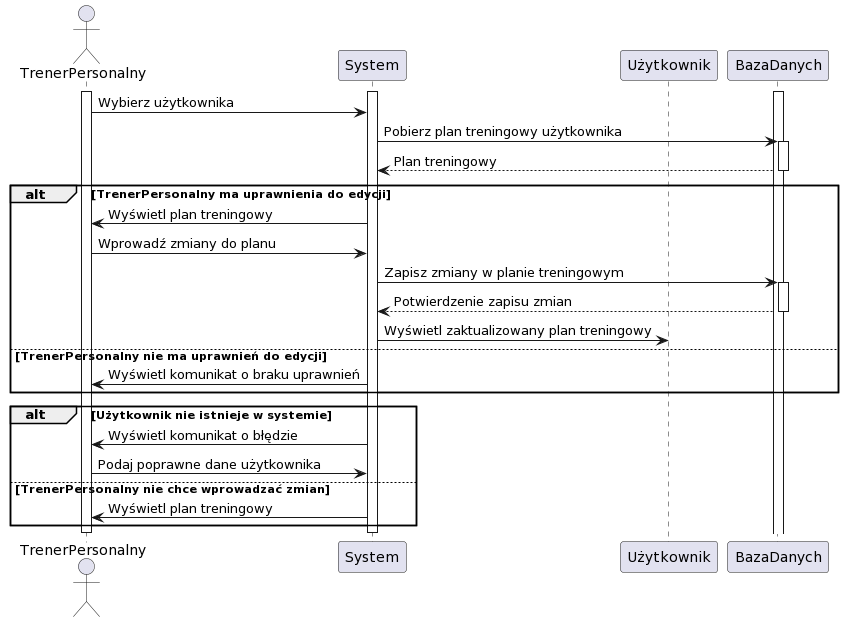
\includegraphics{diagrams/sequence/edycja_planu_treningowego.png}}

{Aktorzy biorący udział: Trener personalny}

{Cel przypadku: Umożliwienie trenerowi personalnemu wprowadzenia zmian
do istniejącego planu treningowego dla danego użytkownika.}

{Warunki początkowe: Trener personalny jest zalogowany do systemu i
posiada uprawnienia do edycji planu treningowego.}

{Warunki końcowe: Zmieniony plan treningowy jest zapisany w systemie i
jest widoczny dla użytkownika.}

{Główny ciąg zdarzeń:}

\begin{enumerate}
\tightlist
\item
  {Trener personalny wybiera użytkownika, którego plan treningowy chce
  edytować.}
\item
  {System wyświetla aktualny plan treningowy dla wybranego użytkownika.}
\item
  {Trener personalny wprowadza zmiany do planu treningowego.}
\item
  {System zapisuje zmiany i aktualizuje plan treningowy dla wybranego
  użytkownika.}
\item
  {System wyświetla potwierdzenie zapisania zmian.}
\end{enumerate}

{Alternatywne ciągi zdarzeń:}

{1a. Trener personalny nie posiada uprawnień do edycji planu
treningowego.}

\begin{itemize}
\tightlist
\item
  {System wyświetla komunikat o braku uprawnień.}
\end{itemize}

{2a. Użytkownik nie istnieje w systemie.}

\begin{itemize}
\tightlist
\item
  {System wyświetla komunikat o błędzie i prosi o podanie poprawnych
  danych.}
\end{itemize}

{3a. Trener personalny nie chce wprowadzać zmian do planu treningowego.}

\begin{itemize}
\tightlist
\item
  {System wyświetla aktualny plan treningowy dla wybranego użytkownika
  bez zmian.}
\end{itemize}

{}

\begin{enumerate}
\setcounter{enumi}{2}
\tightlist
\item
  {Usuń plan treningowy}
\end{enumerate}

{\includegraphics{diagrams/sequence/usun_plan_treningowy.png}}
{Aktorzy biorący udział: Trener personalny}

{Cel przypadku: Umożliwienie trenerowi personalnemu usunięcia planu
treningowego dla danego użytkownika.}

{Warunki początkowe: Trener personalny jest zalogowany do systemu i
posiada uprawnienia do usuwania planu treningowego.}

{Warunki końcowe: Plan treningowy dla danego użytkownika jest usunięty z
systemu.}

{Główny ciąg zdarzeń:}

\begin{enumerate}
\tightlist
\item
  {Trener personalny wybiera użytkownika, którego plan treningowy chce
  usunąć.}
\item
  {System wyświetla aktualny plan treningowy dla wybranego użytkownika.}
\item
  {Trener personalny potwierdza chęć usunięcia planu treningowego.}
\item
  {System usuwa plan treningowy z systemu.}
\item
  {System wyświetla potwierdzenie usunięcia planu treningowego.}
\end{enumerate}

{Alternatywne ciągi zdarzeń:}

{1a. Trener personalny nie posiada uprawnień do usuwania planu
treningowego.}

\begin{itemize}
\tightlist
\item
  {System wyświetla komunikat o braku uprawnień.}
\end{itemize}

{2a. Użytkownik nie istnieje w systemie.}

\begin{itemize}
\tightlist
\item
  {System wyświetla komunikat o błędzie i prosi o podanie poprawnych
  danych.}
\end{itemize}

{3a. Trener personalny nie chce usunąć planu trening}
